\documentclass[10pt]{article}

\AtBeginDocument{%
  \providecommand\BibTeX{{%
    Bib\TeX}}}

\title{NFL Game Outcome Prediction}
\date{}

\usepackage{wrapfig}
\usepackage[skip=7pt plus1pt, indent=0pt]{parskip}
\usepackage{hyperref}
\usepackage[margin=1.0in]{geometry}
\usepackage{cite}
\usepackage{graphicx}
\usepackage{caption}
\usepackage{subcaption}
\usepackage{setspace}
\usepackage{color, colortbl}
\onehalfspacing

\definecolor{Gray}{gray}{0.9}

\AtBeginDocument{%
  \providecommand\BibTeX{{%
    Bib\TeX}}}

\begin{document}

\author{
Hardy Leung\thanks{
Computer Engineering Department, San José State University, \texttt{kwok-shing.leung@sjsu.edu}, MS-AI, 016-711-877} }

\maketitle

\section{Introduction}

American football, or simply football (with apology to soccer fans), has earned
its place as the true national pastime in the United States,
going far beyond its humble origin. Established in 1920,
the National Football League (NFL)
has become one of the most successful sports organizations in the world,
and no description of American culture would be complete without
mentioning the game of football, from the
extravaganza that is the annual Super Bowl, intense rivalries between
college teams, tailgating and BBQs, Monday Night Football, to
everyday idioms borrowed from football -- Hail Mary, moving the goal-post,
punting the problem, getting sacked, and Monday morning quarterbacking.
Simply put, football {\em is} America.

Practically every aspect related to American football is quantitatively
bigger than what most people would expect,
though the estimates vary
widely depending on the scopes and the sources.
According to the Fantasy Sports and Gaming Association\footnote{
\url{https://thefsga.org/industry-demographics/}},
among Americans aged 18 or
older, $24\%$ participate in sports betting, and $20\%$ of participate in
fantasy sports in 2022, with football being by far the most popular category.
In a different study by the research firm Facts and Factors, the
global fantasy sports market size was valued at $24$ billion \textsc{usd}
in 2022,
and projected to reach $45$ billion \textsc{usd} in 2030\footnote{
\url{https://www.fnfresearch.com/news/global-fantasy-sports-market}}.
In a paper published in 2020, Beal, Norman, and Ramchurn \cite{BeNo2020}
 quoted an estimate that is an order of magnitude
bigger,
suggesting that the worldwide sports gambling market was projected to grow
to 565 billion \textsc{usd} by 2022, citing a 2019 report written
by the research firm \texttt{ResearchAndMarkets.com}\footnote{
\url{https://www.businesswire.com/news/home/20190606005537/en/Global-Gambling-Market-Reach-565-Billion-}}. We caution, however, that the figure reported
by the research firm actually including other gambling activities including
casino and lotteries, in which lotteries alone account for $46.1\%$ of
the figure; sports gambling may only be a small portion of the
total amount, possibly more in line with other more conservative estimates.
Regardless,
there is a significant financial stake and opportunity
in improving the accuracy of game outcome prediction.

In truth, Beal et al.~quoted the eye-popping $565$ billion \textsc{usd}
figure partly to motivate their work entitled
``A Critical Comparison of Machine Learning Classifiers to Predict
Match Outcomes in the NFL'' \cite{BeNo2020}.
The authors set out to compare and contrast the performance of different
classification models in order to find one that best predicts the outcome 
of each regular-season NFL football games\footnote{Here, we need to stress the
obvious fact that the prediction uses only information 
prior and up to the beginning of the game. This contracts greatly with
some works that presented amazing results but with the help of
in-game statistics.}.
In their work, Beal and colleagues surveyed
a total of nine machine-learning techniques, including
Support Vector Machine,
$k$-Nearest Neighbors,
Gaussian Process,
Decision Tree,
Random Forest,
AdaBoost,
Na\"ive Bayes, Quadratic Discriminant Analysis (QDA), and Neural Network
(see Table~\ref{table:9}).
The main contribution of their work is an objective and critical evaluation of
the techniques using identical setup. Their dataset is made of the full-game
statistical summary of $1280$
games played by all $32$ NFL teams in the regular season in a
five-year span between $2015$ and $2019$, inclusive\footnote{Each team played
$16$ games in the regular season, so there are a total
of $16$ per
$1280 = 32 \times 16 \times \times 5 \div 2$ games}.

\begin{table}[htbp]
\centering
\begin{tabular}{|c|c|c|}
\hline
Support Vector Machine &
Nearest Neighbors &
Gaussian Process \\
Decision Tree &
Random Forest &
AdaBoost \\ 
Na\"ive Bayes & Quadratic Discriminant Analysis (QDA) & Neural Network \\
\hline
\end{tabular}
\caption{The nine different algorithms that Beal et al.~studied.}
\label{table:9}
\end{table}

We appreciate the head-to-head comparison between different models on
a problem with realistic use cases, and in fact we'll study the paper 
and follow (and extend) their methodology in more details. From now on
we may simply refer to \cite{BeNo2020}
as the {\em Beal paper}, and the authors as
{\em Beal and colleagues}.

\section{Our Motivation}

In this paper,
we shall extend the methodology of Beal and colleagues in three ways: (1) using a
bigger dataset, (2) adding more high-quality features, and (3) including more
models in our analysis.
We want to stress that the foundation of this paper was built on the work by
Beal and colleagues:

\begin{enumerate}
\item They addressed the problem of NFL game prediction head on, using
actual datasets curated from actual games. This is a topic of significant
interest not just to the owners and players, but to a large number of sports fan worldwide
who follow the game, some even religiously.

\item They surveyed nine different machine learning techniques, which
offer a good overview of how these methods performed in a
benchmark that is more sophisticated and richer than many of the
datasets other survey papers focused on. The difficulty of the prediction and the
relevance and groundedness of the problem makes this work highly interesting.
\end{enumerate}

That said, we believe much is left on the table, some of which we will take a closer look at. 
be focusing on.

To begin with, Beal and colleagues claimed that the best performing predictor
has an accuracy of close to $63\%$, in line with the ``Vegas line'' and
the best expert opinion.  In reality,
they adopted a very simplistic model with limited feature selections.
Roughly speaking, there are $21$ distinct concepts such as passing
completions, total yards, etc, for each of the two teams.
These metrics are averaged within the
season as well as across seasons. Together, $84 + 1 = 85$ features are
fed to the classification algorithms being studied. The question is, can we build a better
model, one that can outperform the Vegas line?

As such, we believe there is a significant amount of information that could
have been incorporated into the analysis, such as the QBR rating of the
quarterback, relative strength of teams as measured in other ways, and
playoff consequences. We would like to look into a few of those factors.

Moreover, there are significant and impressive works that are somewhat outside
of the research domain, but may be just as relevant, most notably Nate
Silver's FiveThirtyEight website \cite{Silv2018}. We intended to incorporate
their \textsc{elo}-rating as one of the features, and take some of their
analysis into consideration in crafting better features.
Imagine if we manage to improve the prediction accuracy to just a few percentage
points above the bookmaker's odd, it would have tremendous impact on the sports
betting industry.

\section{Prior Work}

Since the Beal paper was written as a critical evaluation of
different methods of prediction, we did expect the authors to present a more
comprehensive survey-style literature review. Unfortunately, this was not the case and
upon doing our own research, indeed there was an absence of high-quality work. Many
work was published in lesser known journals, and experimental results were not comparable.
Of the prior work Beal and colleagues cited, most were relatively old compared to the actual
year of publication ($2020$). Relatively speaking, the best cited work was
the paper by Boulier and Stekler \cite{Boulier2003}. They also cited a paper by
Landers and Duperrouzel \cite{Landers2018}, but they were mostly concerned with
NFL Fantasy Football games.

The work by Boulier and Stekler \cite{Boulier2003} focused on the comparison between
a logistic regression model and expert predictions. They showed that human prediction
was superior to statistical models, unless the models also incorporate the
carefully crafted ``power scores'' published by New York Times, which measured
the relative abilities of teams, using
objective criteria such as the team’s performance, and
the strengths of schedules \cite{Boulier2003}. If power
scores are included,
then logistic regressions can outperform expert predictions, but still
fall behind the Vegas bookmakers. Beal et al.~cited this work as a comparison, although
it was impossible to do so objectively beyond comparing the reported averages.

Somewhat surprisingly, the research work by Beal and colleagues
has not yet made a broader impact, as it was only cited by
six other publications, albeit given the paper was only published in 2020. Among the few
citations, the one that is the most interesting is 
the paper ``Using Convolutional Neural Network and Candlestick Representation to
Predict Sports Match Outcomes'' by Yu-Chia Hsu \cite{Hsu2021} in 
\textit{Applied Sciences}. Hsu cited the Beal paper as a contrastive comparison to their work
on using a unified and innovative CNN approach to predict game outcomes across different
sports, such as soccer, basketball, and football games. Since the Beal paper required
carefully-crafted
input features specific to the NFL, it is obviously not \textit{immediately} transferable
to other sports. I do not agree with Hsu's assessment that it was a weakness. Nonetheless,
Hsu did generously use a paragraph to describe the approach of Beal and colleagues.

Despite a lack of immediate impact in the research community, we believe Beal et al.~made
a valuable contribution in setting up a baseline for comparison. While we regret that the
authors did not make their source code and dataset available to the public, we did manage
to reproduce at least a portion of their methodologies, though not in actual numbers.
Moreover, the
clean side-by-side comparison between the different methods was tremendously helpful.
If only we could make further progress in improving the accuracy of the NFL predictions,
the paper would have served its purpose.
In fact, ever since Bill Beane stunned the 
world with his data analytics approach to the game of baseball, as described in the
book ``Moneyball'' \cite{Lewis2004}, the world of professional sports have fully embraced 
data science and sports analytics. It would be interesting if the work by Beal
and colleages (and hopefully
our work too) would lead to more research in the area of game outcome prediction.

% Deep neural networks and tabular data: A survey
% \cite{borisov2022deep}

\section{Data}

We start with a discussion of the format of the game for those not familiar with American
football. The NFL is made of $32$ teams grouped in $8$ divisions of $4$ teams each
(see Table~\ref{table:afc-nfc}).
They are the
\textsc{north}, \textsc{east}, \textsc{south}, and \textsc{west} divisions of the
\textsc{afc} (short for American Football Conference), and the
\textsc{north}, \textsc{east}, \textsc{south}, and \textsc{west} divisions of the
\textsc{nfc} (short for National Football Conference).
Each
team plays a total of $17$ regular season games\footnote{Or $16$ games prior to the
$2021$ season.}. Teams compete for eligibility into the playoff, which culminates at the
Super Bowl, played by the two champions of their respective conferences.
Each football game is played in $4$ quarters of $15$ minutes each. Games
that end in a tie at the end of regulation will be decided by additional overtime play. During
regular season, it is possible, but exceptionally rare for a game to end in a tie,
but playoff games are decided by special overtime rules, so one team would
emerge as the eventual
winner. The NFL season starts in September and ends in February of the next
year (for example, the latest Super Bowl played in $2023$ was considered the final
playoff game of the $2022$ season).
Since the
$2021$ season, there are a total
of $32\times 17 \div 2 = 272$ regular season games, with $32$ teams vying for $14$ playoff
spots. A total of $13$ playoff games are played in a single-elimination setting.

\begin{table}[htbp]
\centering
\begin{tabular}{|c|c|c|c|c|}
\hline
\textsc{afc north} & Bengals & Browns & Ravens & Steelers \\
\textsc{afc east} & Bills & Dolphins & Jets & Patriots \\
\textsc{afc south} & Colts & Jaguars & Texans & Titans \\
\textsc{afc west} & Broncos & Chargers & Chiefs & Raiders \\ \hline
\textsc{nfc north} & Bears & Lions & Packers & Vikings \\
\textsc{nfc east} & Commanders & Cowboys & Eagles & Giants \\
\textsc{nfc south} & Buccaneers & Falcons & Panthers & Saints \\
\textsc{nfc west} & 49ers & Cardinals & Rams & Seahawks \\ \hline
\end{tabular}
\caption{The NFL is made of eight divisions of four teams each. During playoff,
$7$ teams from the \textsc{afc} conference will compete for the \textsc{afc}
Championship. Likewise, $7$ teams from the \textsc{nfc} conference will compete for the
\textsc{nfc} Championship. The two conference chmpions will meet at the Super Bowl played
at a neutral site.}
\label{table:afc-nfc}
\end{table}

In a football game, teams aim to score more points than their opponents. Points are scored
by reaching the endzone ($6$ points), kicking the football after touchdown ($1$ point,
better known as the \textsc{pat}), making a two-point conversion in lieu of the \textsc{pat}
($2$ points), and kicking a field goal ($3$ points). The rules of the games can look arcane
and overwhelmingly complicated at times, but mostly we can look at it as a game where the
leader of the offense (the {\em quarterback}) tries to take his team down field by successfully
passing the ball in the air to a receiver, or handing it off to a running back who carries the
ball forward. The game is played on {\em downs}, where the team in possession of the
ball has $4$ tries (first 
down, second down, third down, and fourth down) to convert,
i.e.~to make a total of at least $10$ yards.
If made, it is called a successful {\em conversion}
 (hence the terms third-down and fourth-down conversions),
and the process would start again, with another fresh set of downs. The job of the 
opposing team is
to prevent the offense from making the conversion and from scoring. Strong defense would be
known for their high number of {\em sacks} (roughly, tackling the quarterback before he can
throw a pass) and {\em interceptions} (catching the ball thrown by
the other team).

\subsection{The Beal Paper's Data Source: \texttt{pro-football-reference.com}}

In the era of data anlytics, NFL and many sports networks have collected a large amount of
data and offered said data for further analysis. For example, in a very recent work,
Reyers and Swartz \cite{reyers2023quarterback} used NFL Next-Gen Stats data to track
quarterback options on a frame-by-frame basis, evaluating their options and the quality of
decisions they made. While access to such detailed analysis is out-of-reach for most members
of the research community, it is conceivable that this may change in the near future. That
said, there are multiple sources of NFL data that are available to the general public, either
in the form of a game summary, or play-by-play. In their paper, Beal and colleagues focused on
the statistics of each game, collected by scraping from the website
\url{pro-football-reference.com}. Table~\ref{table:beal-features}
shows the statistics that Beal and colleagues collected from the website, which serves
as the only source of data for their analysis.

\begin{table}
\begin{tabular}{|cc|cc|cc|cc|}
\hline
1 & points scored &
2 & yards gained &
3 & offensive plaays \\
4 & possession lost &
5 & passion completions &
6 & passing yards \\
7 & passing touchdowns &
8 & rushing touchdowns &
9 & rushing yards \\
10 & rushing touchdowns &
11 & expected points scored &
12 & points conceded \\
13 & yards conceded &
14 & defensive plays &
15 & possession gained \\
16 & passing yards conceded &
17 & passing touchdowns conceded &
18 & passing yards conceded \\
19 & rushing touchdowns conceded &
20 & rushing yards conceded &
21 & extra points made \\
\hline
\end{tabular}
\caption{The $21$ statistics captured by Beal and Colleague per game for each playing team.}
\label{table:beal-features}
\end{table}

\subsection{ESPN Game Statistics}

On the other hand,
we were about to find other high-quality datasources, including working API endpoints
 provided by ESPN,
although it is not clear whether those APIs are officially sanctioned by ESPN, or simply
undocumented backdoors. That said, we have
found a large number of scripts that explore those APIs\footnote{
For example,
ESPN Hidden API Docs at 
\url{https://gist.github.com/akeaswaran/b48b02f1c94f873c6655e7129910fc3b},
\texttt{ffscrapr} at
\url{https://ffscrapr.ffverse.com/articles/espn_getendpoint.html},
and ESPN Fantasy Football API at
\url{http://espn-fantasy-football-api.s3-website.us-east-2.amazonaws.com/}. We neither
approve nor condemn the use of these APIs.}.
The collective understanding
of the research community is that accessing the data through those endpoints are tolerated
as long as they are not abused.

For our analysis, we obtain the overall team statistics from ESPN, but via an existing
public Kaggle dataset curated by user \textsc{cviaxmiwnptr}\footnote{
\url{https://www.kaggle.com/datasets/cviaxmiwnptr/nfl-team-stats-20022019-espn}}.
This dataset contains statistics on all games played since the $2002$ season, up to and
including the most recent Super Bowl between Eagles and Chiefs in $2023$. Despite the fact
that the dataset originates from ESPN, the curator (and so do we) noticed that three games
were missing: \textsc{cowboys at commanders} on 2007-12-30, \textsc{panthers at steelers}
on 2010-12-23, and \textsc{buccaneers at falcons} on 2012-01-01. All in all, the dataset
contains a total of $5641$ regular and playoff games over a span of $21$ years. The
statistics that were captured are described in Table~\ref{table:espn-features}. We do
notice a discrepany between the \textsc{pro-football-reference.com} data and the
ESPN data, and indeed the focus is slightly different. However, the key statistics such
as rushing attempts, passing yards, points scored, and completions are all compatible.

\begin{table}
\begin{tabular}{|cc|cc|cc|cc|}
\hline
1 & number of first downs & 2 & number of third downs & 3 & number of fourth downs \\
4 & passing yards & 5 & rushing yards & 6 & total yards \\
7 & number of pass completed & 8 & number of passes attempted & 9 & number of sacks \\
10 & number of rushing attempts & 11 & fumbles & 12 & interceptions \\
13 & turnovers & 14 & penalties & 15 & redzone \\
16 & drives & 17 & defensive stands & 18 & possession \\
19 & score & & & & \\ \hline
\end{tabular}
\caption{The $19$ statistics captured by ESPN.}
\label{table:espn-features}
\end{table}

\subsection{ESPN QBR Ratings}

Perhaps the main reason why we were interested in the ESPN data was the
availability of the QBR metric, which captures an element of the game that simply cannot be
modeled accurately with the passing statistics.
The Total Quarterback Rating, more informally the QBR rating, is 
a metric invented by ESPN to address the shortcoming of commonly
used passer rating metrics. According to Katz and Burke of ESPN,
the QBR metric ``incorporates all of a quarterback’s contributions to winning,
including how he impacts the game on passes, rushes, turnovers and penalties. Also,
since QBR is built from the play level,
it accounts for a team’s level of success or failure on every play to provide the
proper context and then allocates credit to the quarterback and his teammate to
produce a clearer measure of quarterback efficiency.'' \cite{espn2016}. That said,
QBR does have its share of critics, some lamenting QBR as the uglier and more
clumsy sibling of the simpler passing rating formula. To obtain the ESPN dataset, we
relied on the open-source R scripts maintained by user Tom Mock\footnote{
\url{https://github.com/jthomasmock/espnscrapeR}}, who maintained both the scripts to
download the data, as well as a compendium of previously downloaded dataset. The dataset
contains QBR data between the $2006$ season and the $2020$ season, and we
used the script provided to download the data
for the remaining two seasons. The dataset contains a lot of information pertaining
to quarterback plays, such as the number of sacks on the quarterback, but we are primarily
interested in the QBR rating.

Unfortunately, there were a few complications pertaining to the QBR rating. First of all,
the information is incomplete, in that some QBR information was simply missing even when
the starting quarterback has played a full game. This amounts to
$6.04\%$ of the aggregate, which we replaced with league averages.
Second, QBR is by definition a personnel concept, rather than a team concept. We could see
multiple QBR records for a game when a team decided to play multiple QBs in substantial
portion of the games. This happens when the starting quarterback was injured, was pulled
due to underperformance, or sat when the game outcome was already decided. We handled
such situation by simply averaging the QBR ratings. A third complication was that the ESPN
data incorrectly assigned the quarterbacks to their current teams, rather than the teams
they were playing for. For example, in both the $2021$ and $2022$ data, Aaron Rodgers was
misclassified as a Jets quarterback, even though he was just traded to the Jets from
the Packers where he has played his entire professional life. It took quite a bit of
effort and script engineering to fix the problem, but we did\footnote{Namely, we
needed to develop a calendar mapping between game weeks and calendar date, then retrieve
the actual game that the opposing team played against, and that would be the team the
quarterback played for.}.

\subsection{FiveThirtyEight Elo-Rating}

Nate Silver is a well-known statistician known for his expert analysis of the
$2008$ U.~S.~Presidential election where he correctly predicted the election outcome in
forty-nine out of the fifty states. Later, he founded
\texttt{FiveThirtyEight.com}\footnote{\url{https://fivethirtyeight.com}},
a popular website dedicated to the
use of statistical analysis on topics ranging from politics to sports, and anything in between.

We are particularly interested in Silver's \textsc{elo}-ratings of NFL teams, which he 
described very elegantly in a blog post
on the FiveThirtyEight website \cite{Silv2018}. The \textsc{elo}-rating, invented by
physicist and chess player Arpad Elo, was developed initially to rank chess players based
on their performance in comparison to the expected outcome of the matches given the
difference in \textsc{elo}-ratings \cite{elo1978rating}.
Silver adapted the \textsc{elo}-rating to NFL, as the same
analogy applies.
We believe we may be able to take advantage of the \textsc{elo}-rating
as one of the features in our analysis. We get the NFL \textsc{elo}-rating, directly from 
FiveThirtyEight's website\footnote{
\url{https://projects.fivethirtyeight.com/nfl-api/nfl_elo.csv}}. The data provided both
pre-game and post-game \textsc{elo}-ratings, and a quarterback-based adjustment. To be absolutely sure
that we cannot possibly use any unseen data, we only use the post-game \textsc{elo}-rating from
previous games in the analysis. Admittedly, we could have missed some important
signals captured in the difference between the pre-game and post-game \textsc{elo}-ratings -- for
example, if a star quarterback who was injuried for weeks would return in the upcoming game,
we would not have benefited from the updated pre-game \textsc{elo}-ratings. We decided that it would
be best if we work on something simple and more reliable.

\subsection{Data Processing}

With all data available, we perform a substantial amount of data processing to prepare for
the analysis, captured in our $11$-step recipe \texttt{Data.ipynb}:

\begin{enumerate}

\item Setup, and read FiveThirtyEight Elo data. The Elo dataset is used as the
{\em backbone} of the dataset since it does not have any missing data. Elo will be
processed later. We are interested in data since the $2006$ season. There should be a total
of $4576$ entries.

\item Read ESPN team statistics data via Kaggle ($4573$ entries due to the three
missing games).

\item Create dictionaries that allow us to easily refer to any game in 
the ``full game'' format \texttt{home-away|date}. For example,
\texttt{PHI-KC|2023-02-12} refers to the game between home team Philadelphia Eagles and
away team Kansas City Chiefs on February 12, 2023\footnote{This is actually
the most recent Super Bowl played at a neutral site, but Philadelphia got assigned
the home team status.}. We also created ``half game'' lookup of
the form \texttt{<team>|<date>}, for example \texttt{PHI|2023-02-12} and 
\texttt{KC|2023-02-12}.

\item Read ESPN QBR data.

\item Manage the calender. Different datasets refer to the dates differently. For example,
some datasets offer the exact date, but others refer to \textsc{week 1},
\textsc{week 17}, \textsc{wild card}, and \textsc{super bowl}. We manually specify the
date of the first week. There are always $(N+1) + 5$ weeks in a season, where $N$ is the
number of games ($16$ before the $2021$ season, $17$ since), and $N+1$ is the number of
weeks including a bye week for every team. The playoff follows right after the end of the
regular season, with a \textsc{wild card} round, a \textsc{divisional} round, the
\textsc{conference championship}, a bye week, and finally the \textsc{superbowl}.

\item Fix the ESPN QBR fix related to misattributed QB teams.

\item Process FiveThirtyEight Elo data.

\item We create a new dataframe with double the number
of entries but roughly half the number of columns, and cast team stats into this new
dataframe. Given the team stats has $4573$ entries, the new dataframe, called
\texttt{twohalves}, has $4573\times 2 = 9146$ entries.
For example, in the team stats we have an
   entry for \texttt{PHI-KC|2023-02-12} with columns such as \texttt{passing\_yards\_home}
   and \texttt{passing\_yards\_away}. This entry will be split into two new entries, with keys
\texttt{PHI|2023-02-12} and \textsc{KC|2023-02-12}. The home passing yards will go to the
first one, and the away passing yards will go to the second one.

\item Compute league averages on a week-by-week basis.

\item Compute some kind of averages of the statistics, and normalize them to the league
  averages if needed. This is a highly customizable step, and multiple averages can be
created. For example, it could be the average since the beginning of the season, or the
average of the last season, or the average of the last calendar year before the game, or
simply the statistics for the last game. Averages can also be weighted with exponential
decay, so we can put more emphasis on recent games, or games in the current season.
Optionally, the averages are standardized to the
league averages and standard deviation.

\item Finally, combine everything together and rebuild the dataset (and back to $4573$
entries), with a choice of a list of statistics to pull from.
For example, we rebuild the entry for \texttt{PHI-KC|2023-02-12}, using
statistics from (a) the last game, (b) the games played in the same
season, and (c) the game from last season, pulling from both
\texttt{PHI|2023-02-12} and \texttt{KC|2023-02-12}.
\end{enumerate}

This highly sophisticated and choreographed sequence of processing allowed us to
try out different combination of inputs, while ensuring correctness. This was done in order
to avoid data leakage (which could happen if, for example, we normalize the game scores
to the season average). Overall, we have spent a considerable amount of time on making sure
that the data is of the highest quality, and can be easily extensible to cover other
additional datasets.

Now, we are finally ready to run experiments. By default, the tabular dataset we
compiled is made of $4573$ rows of data, between the $2006$ season and $2022$ season (inclusive).
We compute three sets of rolling averages -- \texttt{last-season}, \texttt{this-season}, and
\texttt{last-game} -- each of which is made of $33$ features from each of the two teams.
We also have five info columns named
\texttt{date}, \texttt{home}, \texttt{away}, \texttt{rivalry}\footnote{
For example, \texttt{home} = \texttt{PHI}, \texttt{away} = \texttt{KC}, and \texttt{rivalry} = \texttt{PHI-KC}. The rivalry is technically redundant.},
and \texttt{label} (one if the home team won or tied, and zero if the home team lost).
The total number of columns is $5+33\times 2 \times 3 = 203$.

\section{Experiments}

Beal and colleagues evaluated nine different machine learning
techniques to gain an understanding of how different techniques perform in
what must be a difficult dataset. While there are other works with more
sophisticated methodologies, such as the extensive tabular machine learning survey by
Borisov et al.~\cite{borisov2022deep}, and the impressive work of TabNet by
Arik et al.~\cite{arik2021tabnet}, their results would have been much more convincing
if they were applied to more interesting datasets such as NFL game outcome.

Table~\ref{table:comparison}
is a comparison between the machine learning models they used and the
ones we investigated. In the interest of time, we shall be very brief in describing the
techniques involved.

\begin{table}[htbp]
\centering
\begin{tabular}{|c|c|c|}
\hline
Algorithm & Beal et al.~\cite{BeNo2020} & Our Work \\ \hline
SVM with RBF & Yes & Yes \\
Nearest Neighbors & Yes & Yes ($\star$) \\
Gaussian Process & Yes & Yes \\
Decision Tree & Yes & Yes \\
Random Forest & Yes & Yes \\
AdaBoost & Yes & Yes \\
Na\"ive Bayes & Yes & Yes \\
QDA & Yes & Yes \\
Neural Network & Yes & Yes ($\star$) \\
\rowcolor{Gray}
Logistic Regression & Yes & Yes \\ \hline
XGBoost &  & Yes \\
LightGBM &  & Yes \\
CatBoost &  & Yes \\
Model Tree &  & Yes \\
TabNet &  & Yes \\
Ensemble &  & Yes \\
Elo &  & Yes \\ \hline
\end{tabular}
\caption{The list of machine learning techniques studied by Beal et al.~\cite{BeNo2020}
and by us. Two of the models -- $k$-NN and feed-forward neural network -- were implemented
but their results were not included in our analysis.}
\label{table:comparison}
\end{table}

\begin{description}
\item[\bf Support Vector Machine] -- SVM \cite{cortes1995support}
projects the datapoints to a higher dimensional space
and classsifies the them using a maximum-margin hyperplane.

\item[\bf $k$-Nearest Neighbors] -- $k$-NN \cite{cover1967nearest}
finds the $k$ nearbest neighbors in the feature space using Euclidean distance,
and makes the recommendation using averaging. Although we have experimented with
 the $k$-NN algorithm, it only works on our laptop but not on Google Colab. To
streamline our analysis, we decided to not include $k$-NN in the comparison, since
early indication suggested that it did not perform well, consistent with
the observations made by Beal and colleagues.

\item[\bf Gaussian Process, Quadratic Discriminant Analysis] --
See \cite{williams2006gaussian} and \cite{srivastava2007bayesian}
for more details about these two Bayesian approaches, as we would not be
able do these topics justice.

\item[\bf Na\"ive Bayes] -- This technique \cite{rish2001empirical} makes
strong assumptions about the independence of the features. Contrary to the claim
made by Beal and colleagues, it seems rather far-fetched that such technique 
would perform well given the high correlation between the features (for example, we
expect \texttt{yards\_gained} and \texttt{points\_scored} to be highly correlated).

\item[\bf Decision Tree \cite{breiman2017classification},
Random Forest \cite{breiman2001random},
and ModelTrees \cite{broelemann2018gradient}] --
These are different implementations of decision-tree classifiers, which
usually work very well with tabular data.

\item[\bf AdaBoost \cite{freund1997decision},
CatBoost \cite{prokhorenkova2018catboost}, XGBoost \cite{chen2016xgboost}, LightGBM
\cite{ke2017lightgbm}] -- These are more modern and high performant decission trees that
are based on gradient boosting.


\item[\bf Feed-forward Neural Network and \textsc{tabnet} \cite{arik2021tabnet}] --
\textsc{tabnet} is a relatively new neural network that was designed specifically for
tabular data, and has shown good performance in many benchmarks. Earlier in the
process, we also developed a neural network architecture, but we did not invest
time to fine-tune the hyperparameters. Instead, we shall only show the results from
\textsc{tabnet}.

\item[\bf Ensemble] -- We developed several ensemble methods that combine the
probability estimates and make a group recommendation. Three variations were proposed:
(1) {\bf Vote} -- simple yay/nay voting,
(2) {\bf Sum} -- sum of probabilities, and (3) {\bf Mult} -- product of probabilities.

\item[\bf Elo] -- We also implemented a simple Elo-based model which simply
makes the prediction based on who team having the higher \textsc{elo}-rating.
This is to be used as a
baseline, and to ensure the dataset was not degraded due to improper data transformation.

\end{description}

In the Beal paper, the authors used a dataset of 
$1280$ games from the five consecutive regular seasons from $2015$. Due to the small
sample size, they employed a $10$-fold cross-validation with a $7/3$ train/test split. No
other holdout data was set aside. In comparison, we have a much larger dataset of
$4573$ games, and we evaluated the models based on the very latest data, games in
the most recent three seasons -- $2020$, $2021$, and $2022$. We believe this allows us
to evaluate the models more accurately.

We ran the experiments with $6$ different variations of the tabular data, as shown
in Table~\ref{table:variations}, to experiment with different ways of preparing the tabular
data with different values of $\alpha$ (weekly alpha) and $\epsilon$ (season cliff).
More specifically, if we set $\alpha < 1$,
then during the computation of the rolling averages, games that are
further away will take on a smaller weight.
For
example, if a game happened four weeks ago, it will receive a weight of $\alpha^4$, or
$0.80$ if $\alpha = 0.95$. Season cliff ($\epsilon$)
is another factor that modulates the weights of
games from past seasons. When normalization is turned on, all numbers are normalized to the
rolling league averages up to the current week. When PCA is turned on,
the dimensionlity of the dataset will be reduce to $20$ by default. We can then evaluate
the impact of PCA on the performances of the models.

\begin{table}[htbp]
\centering
\begin{tabular}{|c|c|c|c|c|}
\hline
Variation & Weekly Alpha ($\alpha$) & Season Cliff ($\epsilon$) & Normalization & PCA \\ \hline
1 & 1.00 & 1.00 & \texttt{false} & \texttt{true} \\
2 & 1.00 & 1.00 & \texttt{false} & \texttt{false} \\
3 & 1.00 & 1.00 & \texttt{true} & \texttt{true} \\
4 & 1.00 & 1.00 & \texttt{true} & \texttt{false} \\
5 & 0.95 & 0.50 & \texttt{true} & \texttt{true} \\
6 & 0.95 & 0.50 & \texttt{true} & \texttt{false} \\
\hline
\end{tabular}
\caption{The different variations of data preparation. Weekly alpha
($\alpha$) is the decay factor
that attenuates games that happened further in the past. Season cliff ($\epsilon$) imposes an
additional multipler on games that were played in previous seasons. If normalization is
true, then all statistics are normalized to a rolling league average leading up to the
current week. If PCA is true, then after the data preparation, we apply PCA to reduce the
number of dimensions, defaulted to $20$.}
\label{table:variations}
\end{table}

\subsection{Experiment I: $\alpha=1.00$, $\epsilon = 1.00$, Unnormalized, No PCA}

This represents the default setting without any time-decay of weights. The models have
access to the statistics from the very last game (so it can extract the latest \textsc{elo}-rating),
the current season, and the last season. The performance of the algorithms as measured
in accuracy, precision, recall, and \textsc{f1} score is shown in Table~\ref{table:experiment-I}.

\begin{table}[htbp]
\centering
\begin{tabular}{|c|c|c|c|c|c|}
\hline
Algorithm & Rank & Accuracy & Precision & Recall & \textsc{f1} \\ \hline
Gaussian Process & 16 & 0.4706 & -- & -- & -- \\
QDA & 15 & 0.5294 & 0.5294 & 1.0000 & 0.6923 \\
TabNet & 14 & 0.5376 & 0.5564 & 0.6239 & 0.5882 \\
Decision Tree & 13 & 0.5756 & 0.5929 & 0.6325 & 0.6121 \\
XGBoost & 12 & 0.5864 & 0.5924 & 0.7009 & 0.6421 \\
SVM & 11 & 0.6109 & 0.5878 & 0.8872 & 0.7071 \\
AdaBoost & 10 & 0.5937 & 0.6009 & 0.6923 & 0.6434 \\
Na\"ive Bayes & 9 & 0.5973 & 0.5875 & 0.8034 & 0.6787 \\
LightGBM & 8 & 0.6045 & 0.6034 & 0.7385 & 0.6641 \\
Ensemble (Mult) & 7 & 0.6054 & 0.5959 & 0.7915 & 0.6799 \\
Ensemble (Sum) & 6 & 0.6072 & 0.5984 & 0.7846 & 0.6790 \\
Ensemble (Vote) & 5 & 0.6136 & 0.6065 & 0.7692 & 0.6782 \\
Random Forest & 4 & 0.6109 & 0.6078 & 0.7470 & 0.6702 \\
Model Tree & 3 & 0.6163 & 0.6148 & 0.7368 & 0.6703 \\ \hline
Logistic Regression & 2 & 0.6325 & 0.6211 & 0.7846 & 0.6934 \\ \hline
Elo & 1 & 0.6470 & 0.6696 & 0.6581 & 0.6638 \\
\hline
\end{tabular}
\caption{Experimental I: $\alpha=1.00$, $\epsilon = 1.00$, Unnormalized, No PCA.}
\label{table:experiment-I}
\end{table}

Interestingly, our results are significantly worse than the results presented in the
 Beal paper. Granted, there are many differences between our methodologies: (1) we use
different datasets (ours is between the $2006$ season and the $2022$ season,
and Beal's is between the $2015$ season and the $2019$ season), (2) the features
we used are different (\texttt{pro-football-reference.com} vs
ESPN team stats + FiveThirtyEight \textsc{elo}-rating + QBR),
and (3) the models are different (in addition to
those mentioned in the Beal paper, we have XGBoost, CatBoost, LightGBM, Model Trees,
\textsc{tabnet}, and Ensemble (Ours).

In addition, none of the models matched up to FiveThirtyEight's \textsc{elo}-rating, which achieves
the highest accuracy of $64.7\%$, just as advertised. As we alluded to before, we were
skeptical about the claim that Na\"ive Bayes can significantly outperform other methods.
Indeed, as expected, it was merely middle of the road.

We were disappointed to see that both \textsc{tabnet} and XGBoost underperformed. We believe they
were overfitted. Granted that we did not perform substantial hyper-parameter tuning to
boost their performance, but we did look into controlling their overfitting behaviors. In
any case, if the models cannot perform well out of the box, and was in fact soundly
defeated by basic logistic regression, let's just say that their performances were not stellar.

It is entirely possible that Beal and colleagues use features that are of substantially
higher quality than ours. This remains a possibility, and we regretted that we did not
investigate such scenario with more rigor due to time constraint. That said, I believe 
ESPN + FiveThirtyEight + QBR should match up well with those data from
\texttt{pro-football-reference.com}. At the minimum, our dataset contains one powerful
feature that is the \textsc{elo}-rating, and in fact our result shows that making the decision based
on just that single feature gives us the best result already (see Figure~\ref{fig:elo} for
its per-season performance that our model reported).
We should give credit where credit is due, that Silver and team at FiveThirtyEight did a fantastic
job.

\begin{figure}[htbp]
\centering
\begin{subfigure}{0.61\columnwidth}
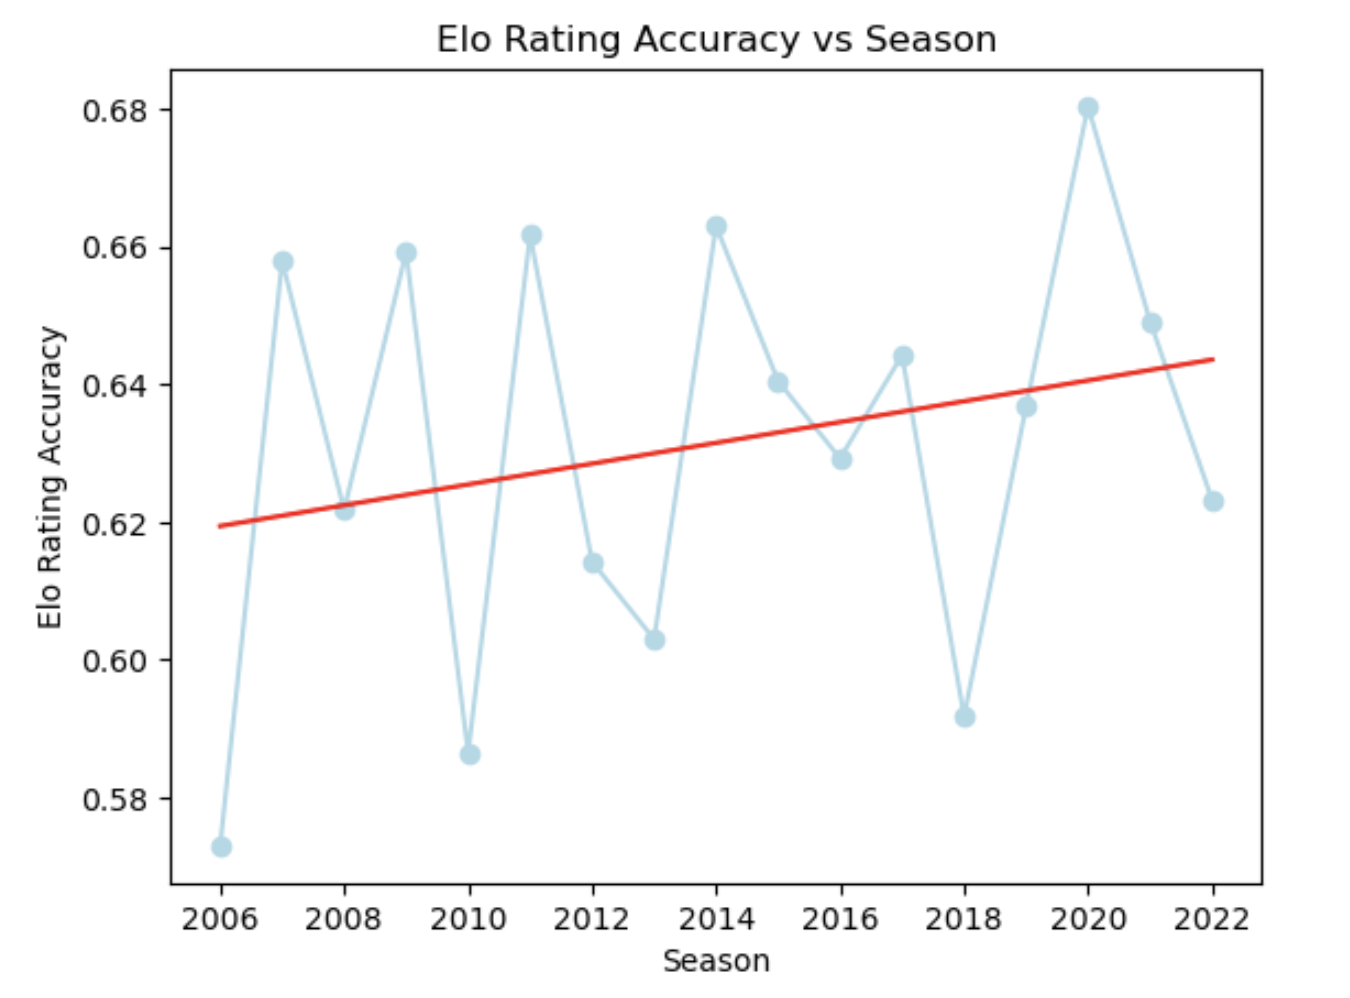
\includegraphics[width=\columnwidth]{elo.png}
\end{subfigure}
\caption{The accuracy of \textsc{elo}-rating as a predictor for NFL game outcomes.}
\label{fig:elo}
\end{figure}


That said, it was surprising that
none other than Logistic Regression was able to pick up these important feature. Perhaps it was
drowned out by the other $200$ features? This is quite likely, and in fact, can fully
explain why logistic regression did so well -- by picking out exactly the right feature.
Figure~\ref{fig:feature-importance} shows the top $15$ most important features selected by
Logistic Regression. In fact, two-third of those features were either \textsc{elo}-ratings or QBRs.

\begin{figure}[htbp]
\centering
\begin{subfigure}{0.81\columnwidth}
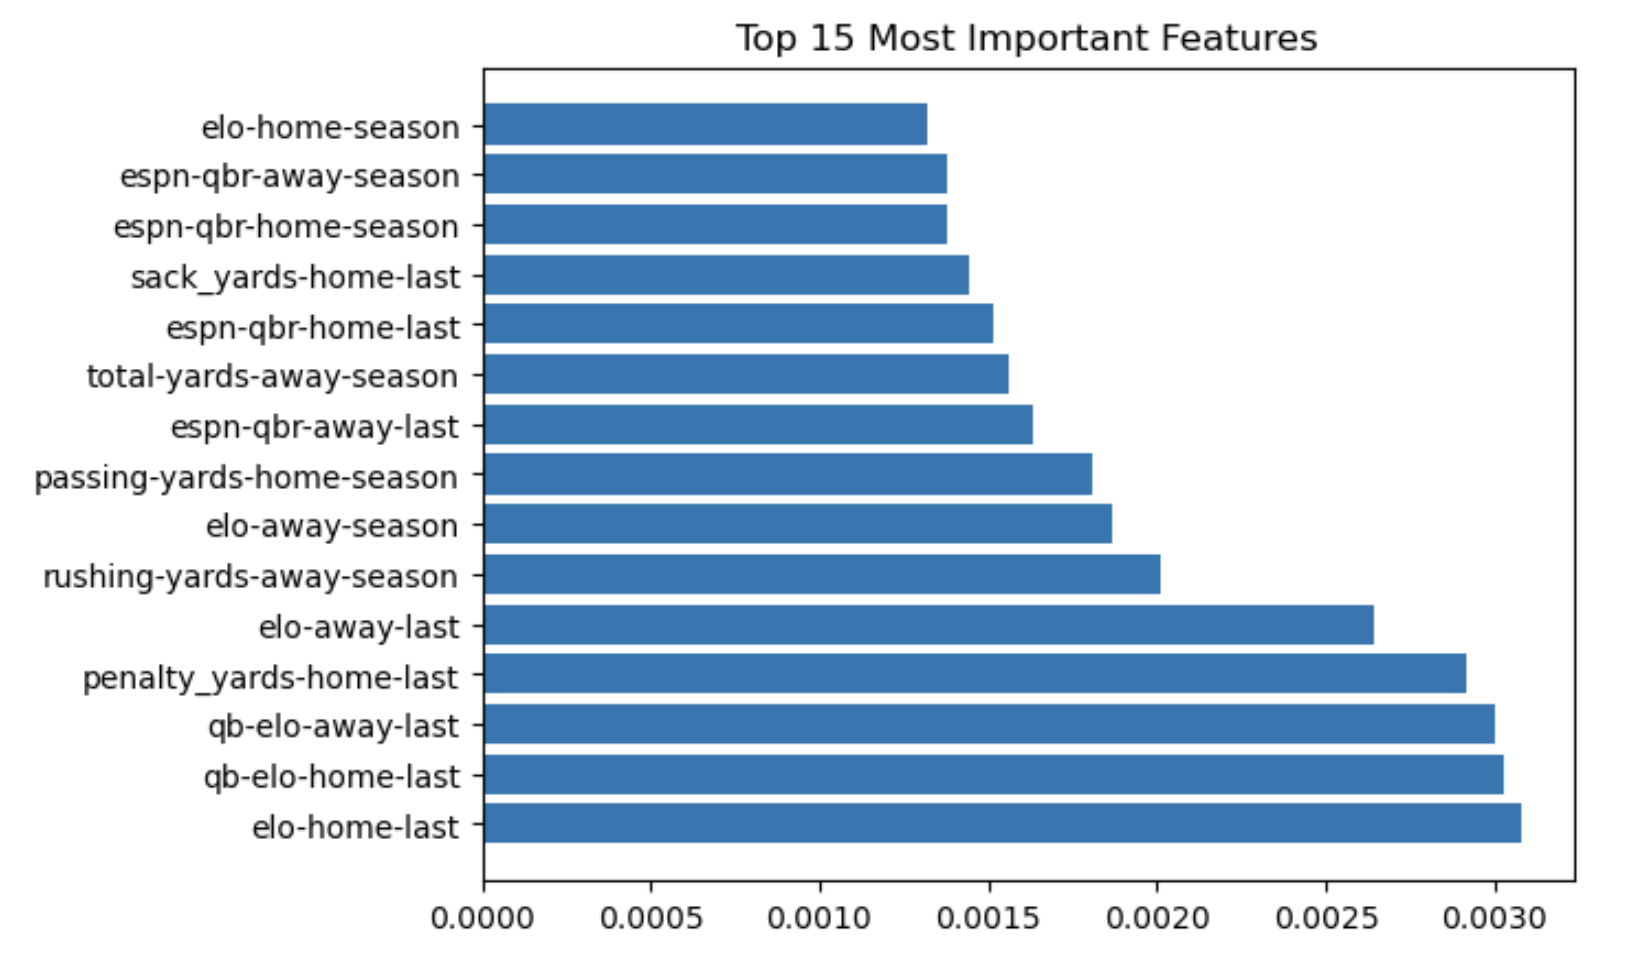
\includegraphics[width=\columnwidth]{feature-importance.png}
\end{subfigure}
\caption{The top-$15$ most importance features.} 
\label{fig:feature-importance}
\end{figure}


\subsection{Experiment II: $\alpha=1.00$, $\epsilon = 1.00$, Unnormalized, PCA}

Is it possible that the our features are too redundant, making it hard for the
models to generalize effectively? In this experiment, we perform principal component analysis
on the dataset prior to running the algorithm\footnote{We simply skip the Elo-based method,
and use the result from the previous experiment.}. The result is
shown in Table~\ref{table:experiment-II}.

\begin{table}[htbp]
\centering
\begin{tabular}{|c|c|c|c|c|c|}
\hline
Algorithm & Rank & Accuracy & Precision & Recall & \textsc{f1} \\ \hline
Gaussian Process & 16 & 0.4706 & -- & -- & -- \\
TabNet & 15 & 0.5357 & 0.5502 & 0.6735 & 0.6057 \\
Decision Tree & 14 & 0.5475 & 0.5687 & 0.6017 & 0.5847 \\
QDA & 13 & 0.6009 & 0.5891 & 0.8137 & 0.6834 \\
Random Forest & 12 & 0.6072 & 0.6024 & 0.7590 & 0.6717 \\
XGBoost & 11 & 0.6090 & 0.6147 & 0.7009 & 0.6550 \\
SVM & 10 & 0.6100 & 0.5925 & 0.8427 & 0.6958 \\
Model Tree & 9 & 0.6163 & 0.6148 & 0.7368 & 0.6703 \\
AdaBoost & 8 & 0.6200 & 0.6132 & 0.7641 & 0.6804 \\
LightGBM & 7 & 0.6217 & 0.6223 & 0.7265 & 0.6703 \\ \hline
Logistic Regression & 6 & 0.6235 & 0.6125 & 0.7863 & 0.6886 \\ \hline
Ensemble (Vote) & 5 & 0.6271 & 0.6183 & 0.7726 & 0.6869 \\
Na\"ive Bayes & 4 & 0.6290 & 0.6061 & 0.8547 & 0.7092 \\
Ensemble (Sum) & 3 & 0.6299 & 0.6219 & 0.7675 & 0.6871 \\
Ensemble (Mult) & 2 & 0.6299 & 0.6222 & 0.7658 & 0.6866 \\
Elo & 1 & 0.6470 & 0.6696 & 0.6581 & 0.6638 \\
\hline
\end{tabular}
\caption{Experimental II: $\alpha=1.00$, $\epsilon = 1.00$, Unnormalized, with PCA.}
\label{table:experiment-II}
\end{table}

PCA helps some models and hurts others. As expected, logistic regression
loses some of its dominance, because other methods were no longer drowned
out as much. In particular,
Na\"ive Bayes did very well, as it thrives when the features are
no longer correlated. Ensemble performed quite admirably,
despite the fact that the inputs are
\textsc{xgboost}, 
\textsc{adaboost}, 
\textsc{tabnet}, 
\textsc{logistic regression}, and
\textsc{lightgbm}. All three ensemble methods outperform all of the
input methods.

\subsection{Experiment III: $\alpha=1.00$, $\epsilon = 1.00$, Normalized, PCA}

We learned that many machine learning models perform better when input is normalized, so
in this experiment, we shall normalize the input to the rolling league averages
(up to that game) see how the models behave.
The result is shown in Table~\ref{table:experiment-III}.

\begin{table}[htbp]
\centering
\begin{tabular}{|c|c|c|c|c|c|}
\hline
Algorithm & Rank & Accuracy & Precision & Recall & \textsc{f1} \\ \hline
QDA & 16 & 0.4823 & 0.5243 & 0.2393 & 0.3286 \\
Na\"ive Bayes & 15 & 0.4842 & 0.5333 & 0.2051 & 0.2963 \\
Gaussian Process & 14 & 0.5294 & 0.5294 & 1.0000 & 0.6923 \\ \hline
Logistic Regression & 13 & 0.5294 & 0.5294 & 1.0000 & 0.6923 \\ \hline
Decision Tree & 12 & 0.5303 & 0.5432 & 0.7094 & 0.6153 \\
XGBoost & 11 & 0.5665 & 0.5673 & 0.7641 & 0.6511 \\
SVM & 10 & 0.5709 & 0.5709 & 1.0000 & 0.7269 \\
Model Tree & 9 & 0.5744 & 0.5735 & 0.9929 & 0.7271 \\
LightGBM & 8 & 0.5756 & 0.6086 & 0.5556 & 0.5809 \\
Random Forest & 7 & 0.5765 & 0.5990 & 0.6051 & 0.6020 \\
Ensemble (Vote) & 6 & 0.5819 & 0.5718 & 0.8376 & 0.6796 \\
TabNet & 5 & 0.5919 & 0.5876 & 0.7675 & 0.6657 \\
Ensemble (Mult) & 4 & 0.5919 & 0.5840 & 0.7966 & 0.6739 \\
AdaBoost & 3 & 0.5937 & 0.5852 & 0.7983 & 0.6753 \\
Ensemble (Sum) & 2 & 0.5937 & 0.5852 & 0.7983 & 0.6753 \\
Elo & 1 & 0.6470 & 0.6696 & 0.6581 & 0.6638 \\
\hline
\end{tabular}
\caption{Experimental III: $\alpha=1.00$, $\epsilon = 1.00$, Normalized, with PCA.}
\label{table:experiment-III}
\end{table}

We got very interesting results when we normalize the
feature values to the league averages. Almost all
models performed worse, with the exception of \textsc{tabnet},
which rose to the top together with the ensemble models,
seemingly validating the importance of standardization for
neural models.
Logistic Regression performed very poorly compared
to previous results. Frankly, we did not want to make further
interpretation because it was not at all clear to us what was
happening.

\subsection{Experiment IV: $\alpha=0.95$, $\epsilon = 0.50$, Unnormalized, No PCA}

In this section, we shall vary $\alpha$ and $\epsilon$ so games that are further
in the past are weighted less. The result is shown in Table~\ref{table:experiment-IV},
which is best compared to the first experiment shown in Table~\ref{table:experiment-I}.
The experimental results did not show substantial movement in any model. The ensembles
are slightly improved, possibly because of the better quality of models.

\begin{table}[htbp]
\centering
\begin{tabular}{|c|c|c|c|c|c|}
\hline
Algorithm & Rank & Accuracy & Precision & Recall & \textsc{f1} \\ \hline
 QDA & 16 & 0.4697 & 0.4935 & 0.0650 & 0.1148 \\
 Gaussian Process & 15 & 0.4706 & -- & -- & -- \\
 TabNet & 14 & 0.5403 & 0.5399 & 0.8906 & 0.6723 \\
 Decision Tree & 13 & 0.5692 & 0.5932 & 0.5932 & 0.5932 \\
 AdaBoost & 12 & 0.5954 & 0.6117 & 0.6462 & 0.6284 \\
 Na\"ive Bayes & 11 & 0.6018 & 0.5926 & 0.7932 & 0.6784 \\
 XGBoost & 10 & 0.6027 & 0.6127 & 0.6786 & 0.6440 \\
 LightGBM & 9 & 0.6063 & 0.6130 & 0.6957 & 0.6517 \\
 SVM & 8 & 0.6090 & 0.5870 & 0.8821 & 0.7049 \\
Ensemble (Vote) & 7 & 0.6136 & 0.6079 & 0.7607 & 0.6758 \\
Ensemble (Mult) & 6 & 0.6235 & 0.6125 & 0.7863 & 0.6886 \\
Ensemble (Sum) & 5 & 0.6235 & 0.6125 & 0.7863 & 0.6886 \\
 Random Forest & 4 & 0.6235 & 0.6181 & 0.7556 & 0.6780 \\
 Model Tree & 3 & 0.6262 & 0.6229 & 0.7453 & 0.6786 \\ \hline
 Logistic Regression & 2 & 0.6271 & 0.6151 & 0.7897 & 0.6916 \\ \hline
Elo & 1 & 0.6470 & 0.6696 & 0.6581 & 0.6638 \\
\hline
\end{tabular}
\caption{Experimental IV: $\alpha=0.95$, $\epsilon = 0.50$, Unnormalized, No PCA.}
\label{table:experiment-IV}
\end{table}

\section{Conclusion}

In this paper, we have evaluated many models to predict NFL game
outcomes. We started with the foundation laid by Beal and colleagues,
extended their results in several ways:

\begin{itemize}

\item We acquired a more comprehensive and complete dataset that
starts in the $2006$ season up until now.  Our model is $350\%$ the size of
the Beal model.

\item We sought to incorporate key statistics, including \textsc{elo}-ratings from
FiveThirtyEight and ESPN QBR ratings, into our analysis, which
was proven to be fruitful.

\item We evaluated over a dozen different models, including all
models seen in the Beal paper, as well as state-of-the-art models
such as \textsc{xgboost}, \textsc{lightgbm}, and \textsc{tabnet}.

\item We developed an ensemble model that was able to offer better
predictions.

\item We developed a robust data processing that allowed us to experiment
with different ways of packaging and averaging the features in
a modular fashion.

\item We have studied the impact of normalization, dimensionality
reduction, and weight decay on the performance of the models,
and offered observations whenever possible.

\end{itemize}

Although we were somewhat disappointed by the relatively poor performance of our models,
this is nonetheless a worthy exercise.
We conclude by pointing out that there is still significant
opportunity in analyzing and optimizing the models. In fact, we totally believe it is
entirely possible to reach a $70\%$ prediction accuracy, although doing so would call for
better techniques beyond full-game statistics.
The world of
sports analytics and game outcome analysis is wide open, and we look forward to 
more inspired work in this area.

\bibliographystyle{acm}
\bibliography{report}

\end{document}
